\chapter{Pharmacokinetic modelling}
\label{chapter:pk}

The ideal output obtained from DCE-MRI analysis would be some reliable quantitative physiological parameters of the tissue under examination. 

PK models have very wide clinical application: from estimating the optimal drug dose to determining safe working environment while working with toxins  \cite{gerlowski1983physiologically}.
Given the fact that the contrast agent used in DCE-MRI examination can be considered as a substance flowing through the organism, pharmacokintetic modelling can also be used in analysis of so obtained data.   
This approach, called the parametric one, is based on fitting mathematical model to acquired tissue concentration time courses. In this way, the quantitative parameters can be assessed, which cannot be overestimated while evaluating the tissue function. 


\section{Arterial Input Function}
All PK models require the qquistition Arterial Input Function


\begin{comment}
The time-dependent distribution and disposition of a substance in a living system can be described by phamacokinetic (PK) models~\cite{gerlowski1983physiologically}. They aim to characterise a physiologic system by decomposing them into interacting compartments. Every of them is a homogenous, well-mixed space with the uniform tracer distribution \cite{PMID:20540902}.









The compartment PK models decribe complex
blood-tissue exchanges and their theory
is based on the differential mass balance equations
[29]. An example of the system decribed
by two compartments is presented on Figure 5.
	


\end{comment}

\begin{figure}
		\centering
		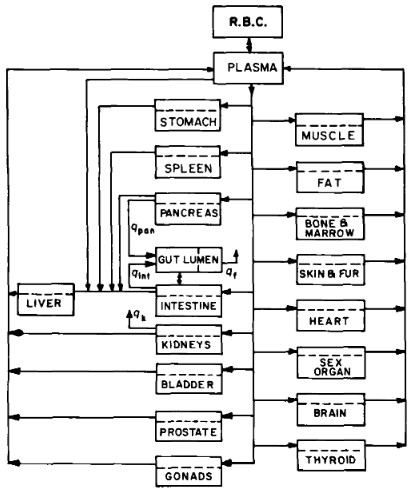
\includegraphics[height = 10cm]{scheme}
		\caption [DCE-MRI enhacement patterns]{Different DCE-MRI enhacement patterns \cite{khalifa2014models}}
		\label{fig:pk_draft}
	\end{figure}